\section{Figure example}\label{sec:figure}

A simple figure example is shown as figure \ref{fig:bivariate}.

\begin{figure}[!htb]
\centering
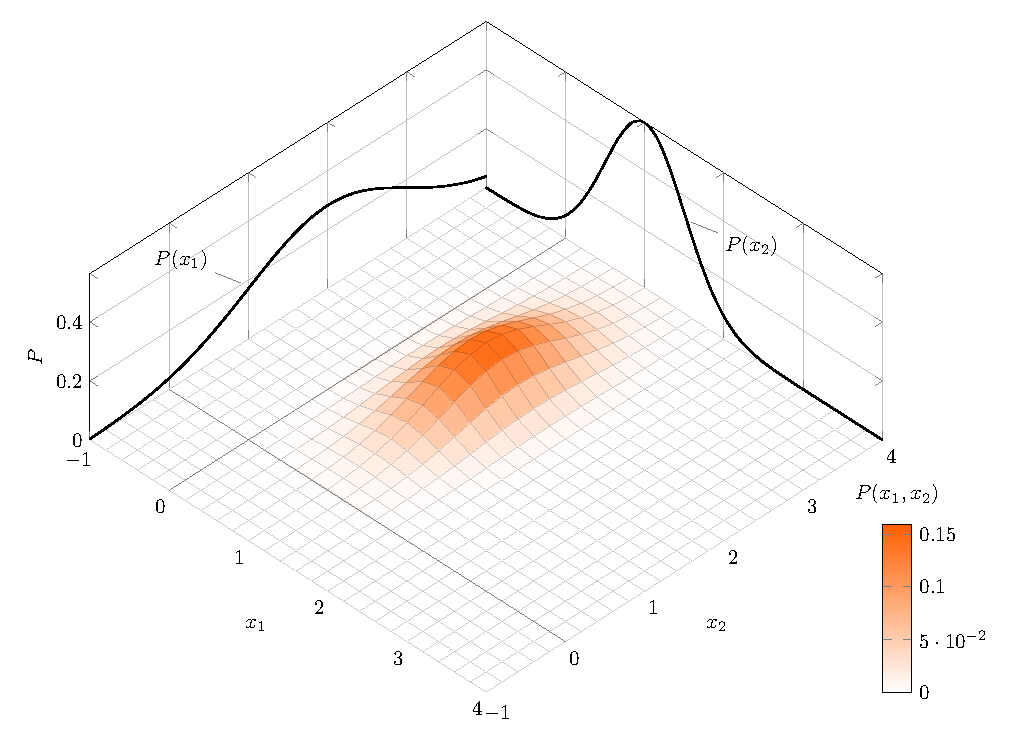
\includegraphics[width=0.6\textwidth]{bivariate-normal-distribution.pdf}
\caption{Figure example}\label{fig:bivariate}
\end{figure}

For two independent side-by-side figures, you can use two minipages inside a figure enviroment. Here's an example, shown as figure \ref{fig:h_example_19} and \ref{fig:h_example_82}.
\begin{figure}[!htb]
\begin{minipage}[t]{0.5\linewidth}
\centering
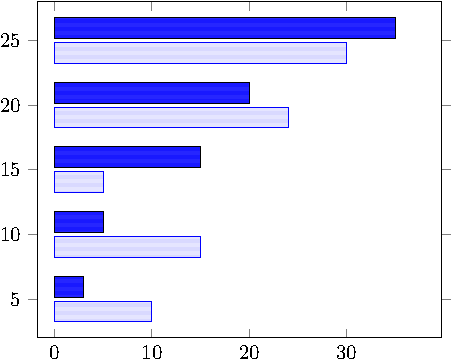
\includegraphics[width=0.8\textwidth]{h_example_19.pdf}
\caption{Figure example}\label{fig:h_example_19}
\end{minipage}
\begin{minipage}[t]{0.5\linewidth}
\centering
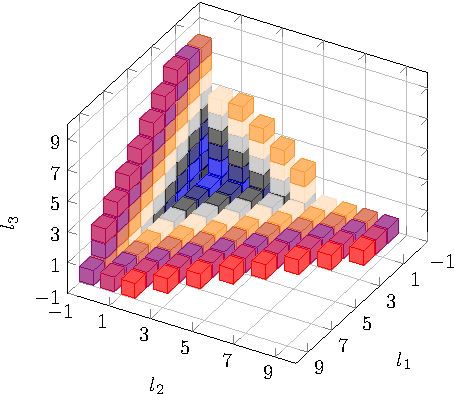
\includegraphics[width=0.8\textwidth]{h_example_82.pdf}
\caption{Figure example}\label{fig:h_example_82}
\end{minipage}
\end{figure}
